\documentclass{article}
\usepackage{amsmath}
\usepackage{amsfonts}
\usepackage{geometry}
\usepackage{graphicx}
\geometry{a4paper,scale=0.75}
\title{Solution for Exercise sheet 1}
\author{You Zhou}
\date{}
\begin{document}
\maketitle
\paragraph{Exercise 1.1}For a fixed integer $j,$ let $\{e_i^j\}_i$ denote the set of $j$-cells of $X,$  let $\Phi_i^j\colon D^{j}\rightarrow X^{j}$ be the characteristic map of $e_i^j.$ Then a map $f\colon X\rightarrow Y$ is the union of maps
\[f_{ij}:=f|_{\overline{e_i^j}}\circ\Phi_i^j\colon D^j\rightarrow Y.\]
Viewing $D^j$ as the upper half of $S^j$, we can define maps
\begin{align*}
  \widetilde{f_{ij}}\colon S^{j} &\rightarrow Y \\
  (x_0,\,\ldots,\,x_n) &\mapsto \begin{cases}
   f_{ij}(x_0,\,\ldots,\,x_n),\,&\text{if } x_n\geq0\\
   f_{ij}(x_0,\,\ldots,\,-x_n),\,&\text{if }x_n<0
   \end{cases}
\end{align*}
This map is continuous and can be view as an element of $\pi_j(Y,y)$ for some $y_{ij}\in Y.$ We then show that two maps $f,\,g\colon X\rightarrow Y$ are homotopic if and only if for all $i,\,j,\,\widetilde{f_{ij}}$ and $\widetilde{g_{ij}}$ are homotopic and the following condition is satisfied:
\begin{quote}
  Let $\widetilde{H_{ij}}\colon S^j\times[0,1]\rightarrow Y$ be the continuous map such that $\widetilde{H_{ij}}(x,0)=\widetilde{f_{ij}}(x)$ and $\widetilde{H_{ij}}(x,1)=\widetilde{g_{ij}}(x).$ If there exist some $i,j,i',j'$ and $x\in D^j,y\in D^{j^{\prime}}$ such that $\Phi_i^j(x)=\Phi_{i'}^{j'}(y),$ then $\widetilde{H_{ij}}(x,t)=\widetilde{H_{i'j'}}(y,t)$ for all $t\in[0,1].$
\end{quote}

For one thing, let $H\colon X\times[0,1]\rightarrow Y$ be a continuous map such that $H(x,0)=f(x)$ and $H(x,1)=g(x).$ By restricting $H$ to $\overline{e_i^j}$ and then use the method of defining $\widetilde{f_{ij}}$ from $f_{ij},$ we can get the required maps $\widetilde{H_{ij}}.$

For another, let $\widetilde{H_{ij}}\colon S^j\times[0,1]\rightarrow Y$ be continuous maps with $\widetilde{H_{ij}}(x,0)=\widetilde{f_{ij}}(x)$ and $\widetilde{H_{ij}}(x,1)=\widetilde{g_{ij}}(x)$ for all $i$ and $j$ and satisfying the condition above. Define
\begin{align*}
  H\colon X\times[0,1] & \rightarrow Y \\
  (x,t) & \mapsto \widetilde{H_{ij}}(x,t),\text{ for }x\in\Phi_i^j(D^j)
\end{align*}
Then the condition ensures that $H$ is well-defined. This $H$ is also continuous, so this proves our claim.

Note that a homotopy class of $\widetilde{f_{ij}}$ is an element of $\pi_j(Y,y_{ij})$ for some $y_{ij}\in Y.$ So the homotopy class of $\widetilde{f_{ij}}$ has only finitely many possibilities, and so does the homotopy class of $f$.
\paragraph{Exercise 1.2}
\subparagraph{(a)}To give the map explicitly we use coordinates. Set
\begin{align*}
  S^n & :=\{(x_0,\,\ldots,\,x_n)\in\mathbb{R}^{n+1}\mid x_0^2+\cdots+x_n^2=1\} \\
  S^n\vee S^n & :=\{(x_0,\,\ldots,\,x_n)\in\mathbb{R}^{n+1}\mid (x_0\pm\frac{1}{2})^2+\cdots+x_n^2=\frac{1}{4}\}
\end{align*}
The pinch map then can be given by
\[p(x_0,\,\ldots,\,x_n)=\left(x_0,\,\sqrt{\frac{|x_0|}{1+|x_0|}}x_1,\,\ldots,\,\sqrt{\frac{|x_0|}{1+|x_0|}}x_n\right),\]
which is clearly continuous. In this coordinate system $q_1$ can be given by
\begin{align*}
  q_1\colon S^n\vee S^n & \Rightarrow S^n \\
  (x_0,\,\ldots,\,x_n) & \mapsto
  \begin{cases}
   (2x_0+1,\,2x_1,\,\ldots,\,2x_n),\,&\text{if } x_0\leq0\\
   (1,\,0,\,\ldots,\,0),\,&\text{if }x_0>0
   \end{cases}
\end{align*}
Both maps and their composition are illustrated for $n=1$ in the figure below. A homotopy
\[H\colon S^n\times[0,1]\rightarrow S^n\]
from $\rm{id}|_{S^n}$ to $q_1\circ p$ can be described as follows. Let $x\in S^n$ and $C$ be the geodesic from $(-1,\,0,\,\ldots,\,0)$ to $(1,\,0,\,\ldots,\,0)$ and passing through $x.$ Let $f$ be a homeomorphism from $[0,1]$ to $C$ that sends $0$ to $(-1,\,0,\,\ldots,\,0)$ and 1 to $(1,\,0,\,\ldots,\,0).$ Let
\[\tilde{H}\colon [0,1]\times[0,1]\rightarrow[0,1]\]
be a homotopy of $[0,1]$ such that 
\[H(-,0)=\mathrm{id},\,H([0,\frac{1}{2}],1)=[0,1] \text{ and that }\]
\[H(0,t)=0,\,H(1,t)=1\text{ for all }t\in[0,1].\]
Then
\[H(x,t)=f\circ\tilde{H}(f^{-1}(x),t)\]
is the required homotopy. The case for $q_2\circ p$ is similar.
\begin{figure}[ht]
  \centering
  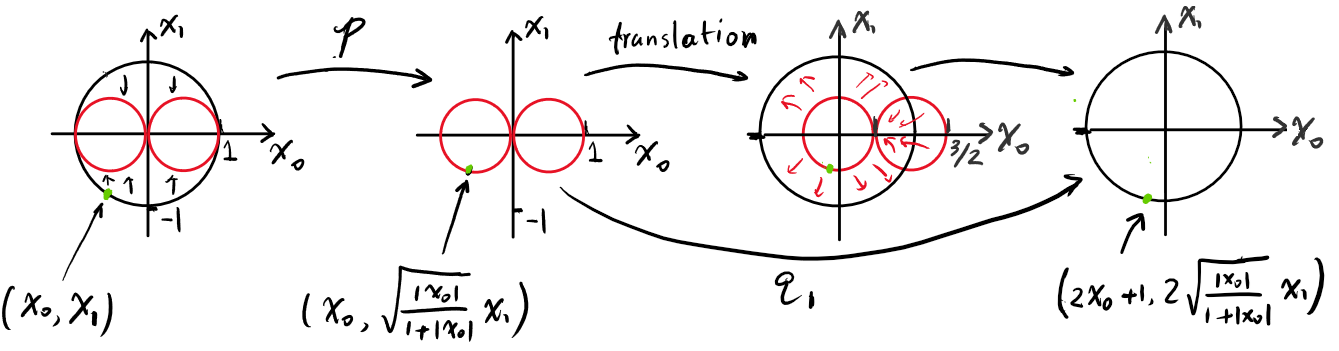
\includegraphics[width=15cm]{ES1_1.png}
  \caption{maps $p$ and $q_1,\,n=1$}
\end{figure}
\subparagraph{(b)}By part (a) we have
\[(q_1\circ p)_*=(q_2\circ p)_*=\mathrm{id}\text{ on }H_n(S^n,A).\]
Thus
\begin{align*}
  (i_1)_*+(i_2)_* & =(i_1)_*\circ (q_1)_*\circ p_*+(i_2)_*\circ (q_2)_*\circ p_* \\
   & =((i_1\circ q_1)_*+(i_2\circ q_2)_*)\circ p_* \\
   & =(\mathrm{id})_*\circ p_*\quad\text{(This step is explained below.)}\\
   & =p_*.
\end{align*}
Let us explain why $(i_1\circ q_1)_*+(i_2\circ q_2)_*=\mathrm{id}_*$ on $H_n(S^n\vee S^n, A).$ Using the coordinate expression of $S^n\vee S^n$ as above, we define
\[B_1:=\{(x_0,\,\ldots,\,x_n)\in S^n\vee S^n\mid x_0\leq \frac{1}{4}\}\text{ and }B_2:=\{(x_0,\,\ldots,\,x_n)\in S^n\vee S^n\mid x_0\geq -\frac{1}{4}\}.\]
Then we have the Mayer-Vietoris sequence (note that $B_1\cup B_2=S^n\vee S^n$)
\[\cdots\rightarrow H_n(B_1\cap B_2,A)\rightarrow H_n(B_1,A)\oplus H_n(B_2,A)\overset{j_*}\rightarrow H_n(S^n\vee S^n)\rightarrow H_{n-1}(B_1\cap B_2,A)\rightarrow\cdots\]
and $j_*=(i_1)_*+(i_2)_*.$ It is clear that
\[((q_1)_*+(q_1)_*)\circ((i_1)_*+(i_2)_*)=\rm{id}\]
So
\[((i_1)_*+(i_2)_*)\circ((q_1)_*+(q_1)_*)\circ((i_1)_*+(i_2)_*)=(i_1)_*+(i_2)_*.\]
Since $B_1\cap B_2$ is contractible, we know that $j_*$ is an isomorphism and composing with $j_*^{-1}$ on both sides gives us the required result.
\subparagraph{(c)}Suppose that $p_1,\,p_2\colon S^n\rightarrow S^n\vee S^n$ are two pinch maps. They can be seen as elements of $\pi_n(S^n\vee S^n, x_0).$ Since $S^n\vee S^n$ is $(n-1)$-connected, we have the Hurewicz map
\[h\colon\pi_n(S^n\vee S^n, x_0)\overset{\sim}\rightarrow H_n(S^n\vee S^n,\mathbb{Z}).\]
By part (b), we know that $h(p_1)=h(p_2).$ Since $h$ is an isomorphism, it follows that $p_1$ and $p_2$ are homotopic as based maps.
\paragraph{Exercise 1.3}Let
\[\partial\colon\pi_2(X,A,x_0)\rightarrow\pi_1(A,x_0)\]
be the group homomorphism given by restricting a map $(I^2,\partial I^2, J^1)\rightarrow(X,A,x_0)$ to $I,$ which can be viewed as $I\times\{0\}\subset\partial I^2.$ Take $h_1,h_2$ in $\pi_2(X,A,x_0),$ then we can construct a homotopy from $h_1h_2h_1^{-1}$ to $(\partial h_1)\star h_2$ as illustrated in the following picture.
\begin{figure}[ht]
  \centering
  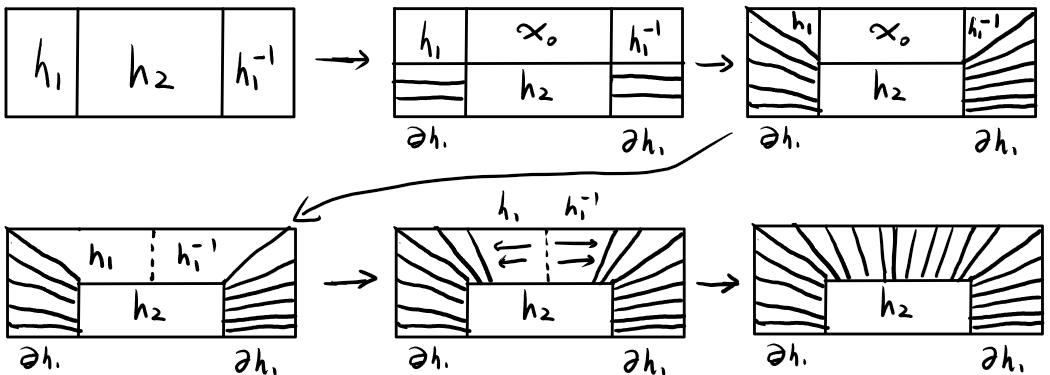
\includegraphics[width=13cm]{ES1_2.png}
  \caption{homotopy from $h_1h_2h_1^{-1}$ to $(\partial h_1)\star h_2$}
\end{figure}

Here in the fourth picture the dotted line is mapped to $x_0.$ In the fifth picture the images of points in the interior of the dotted line are moving from $x_0$ to the corresponding point in $\partial h_1.$ From this we know that in $\pi_2(X,A,x_0)^{\dagger},$
\[h_1h_2h_1^{-1}=(\partial h_1)\star h_2=h_2.\]
\end{document} 